\section{Experimental Evaluation}
\label{sec:eval}
We present a comprehensive evaluation of state-of-the-art agents and LLMs on \sysname{}.
Overall, the results show that \sysname presents a significant challenge for current agents and models.
It also provides a clear ladder of difficulties (e.g., \cref{fig:success_rate_vs_gt_poc_len}), differentiating agents' and models' cybersecurity skills, which will be useful for progress tracking.

\rbtl{Evaluating state-of-the-art agents and LLMs in non-thinking mode on full \sysname{} requires approximately \$3,000 in API credits.
To enable more lightweight and budget-friendly evaluations, we also provide a randomly selected subset of 300 instances ($\sim$20\% of the entire benchmark).}
More details about experimental setup, including prompts, compute, agent configurations, and model versions, are provided in~\cref{app:setup}.
Specific setups and results for each experiment are discussed separately.
Unless explicitly specified, we use difficulty level 1 (our primary reproduction task).

\paragraph{Backbone LLMs Differ Significantly in Reproduction Success Rate}
We select eleven state-of-the-art LLMs from three categories: (i) General-purpose closed-source LLMs: \gptiv{}~\citep{openai_gpt4.1}, \gptv{}~\citep{openai_gpt5}, o4-mini~\citep{openai_o3_o4mini}, \claudeiii{}~\citep{claude37sonnet}, \claudeiv{}~\citep{claudesonnet4}, and Gemini-2.5-Flash~\citep{gemini25flash}; (ii) General-purpose open-weight LLMs: Qwen3-235B-A22B~\citep{qwen3} and DeepSeek-V3~\citep{deepseekv3}; (iii) Specialized LLMs optimized for \openhands~\citep{openhands} to solve \swebench{}~\citep{jimenez2024swebench}: SWE-Gym-32B~\citep{swegym}, R2E-Gym-32B~\citep{r2egym}, and OpenHands-LM-32B~\citep{openhands_lm32b}.
In this experiment, we disable the thinking mode to reduce cost in this experiment, except for o4-mini, which does not support disabling thinking, and \gptv{}, for which minimal reasoning effort is used.
We adopt \openhands{} as the agent scaffold~\citep{openhands} of these LLMs
\rbtl{with a maximum of 100 iterations per task.}

Overall, \claudeiv achieves the best result with a success rate of 17.9\%, followed by \claudeiii and \gptiv.
Specialized models such as SWE-Gym-32B, R2E-Gym-32B, and OpenHands-LM-32B, despite their strong result on SWE-bench~\citep{jimenez2024swebench}, demonstrate poor generalization on \sysname, with success rates $\leq$2.0\%.
\cref{fig:diff_models} illustrates the results of different LLMs.
This demonstrates the complementarity between SWE-bench and \sysname.
\begin{wrapfigure}{r}{.52\textwidth}
    \centering
    \vspace{-4mm}
    \rbtlframe{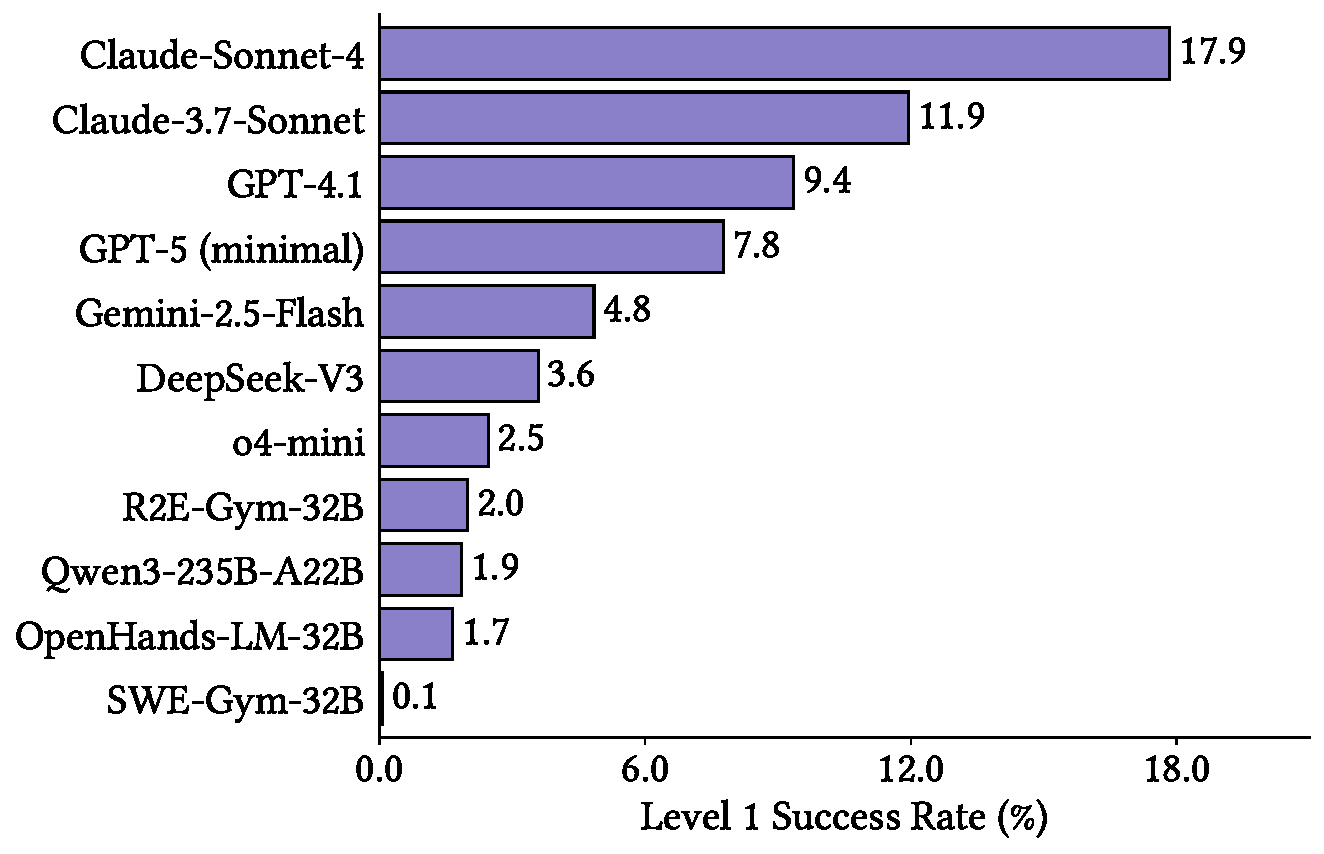
\includegraphics[width=\linewidth]{figures/different_models.pdf}}
    \vspace{-6mm}
    \caption{Results of various LLMs with \openhands.}
    \vspace{-4mm}
    \label{fig:diff_models}
\end{wrapfigure}
\rbtl{
Notably, o4-mini shows a relatively low success rate.
Upon further inspection, we found that o4-mini often conservatively requests user confirmation and prematurely terminates the execution.%, disrupting \openhands' automatic approval mechanism.
We do not observe this pattern in other models, highlighting the need for agent developers to handle such model-specific behaviors to maximize agent utility and robustness.}
\rbtl{The union of all results yields a 27.2\% success rate, revealing the low overlap in the tasks successfully completed by different models.}
\rbtl{Additional results in~\cref{app:results} show that balanced resampling across projects and crash types maintains consistent conclusions.}

\begin{wrapfigure}[10]{r}{.4\textwidth}
    \vspace{-4.2mm}
    \centering
    \rbtlframe{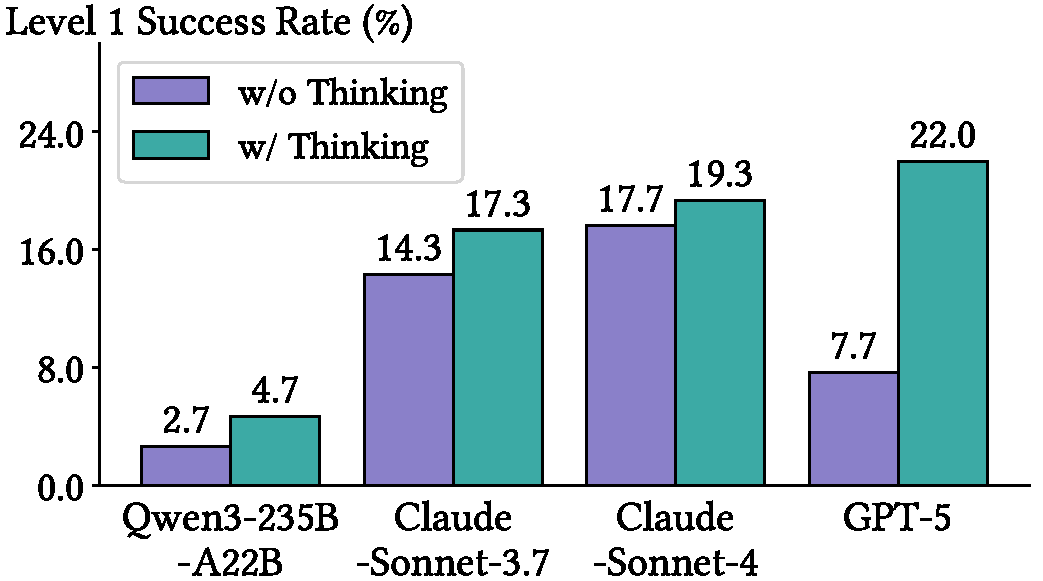
\includegraphics[width=\linewidth]{figures/thinking_vs_nonthinking.pdf}}
    \vspace{-5.5mm}
    \caption{With and without thinking.}
    \label{fig:thinking}
\end{wrapfigure}
\paragraph{Thinking Mode Improves Success Rate}
We compare thinking and non-thinking modes using Qwen3-235B-A22B, \gptv, \claudeiii, and \claudeiv on the 300-instance subset.
\rbtl{We allow more output tokens for thinking mode while applying the same 100 iteration limit to both modes (detailed in~\cref{app:setup}).}
As illustrated in~\cref{fig:thinking}, while the thinking mode yields modest gains over other models, it increases \gptv's success rate from 7.7\% (with minimal reasoning) to 22.0\% (with high reasoning), surpassing \claudeiv.
This phenomenon is consistent with GPT-5's results for other benchmarks~\citep{openai_gpt5}.

\paragraph{Different Agents Show Distinctive Behaviors Despite Similar Success Rates}
We evaluate two general-purpose coding agents, \openhands{}~\citep{openhands} and OpenAI \codex{} CLI~\citep{openai_codex}, alongside two cybersecurity agents for solving CTF problems, \enigma{}~\citep{enigma} and \cybench{} agent~\citep{cybench}.
\rbtl{We apply maximum budget and iteration constraints that yield an average cost of approximately \$2.0 per task for each agent.}
We use \gptiv{}~\citep{openai_gpt4.1} as the backbone LLM, because it achieves a strong balance between cost, rate limits, and success rates.

\begin{wrapfigure}{r}{.35\textwidth}
    \vspace{-4mm}
    \centering
    \rbtlframe{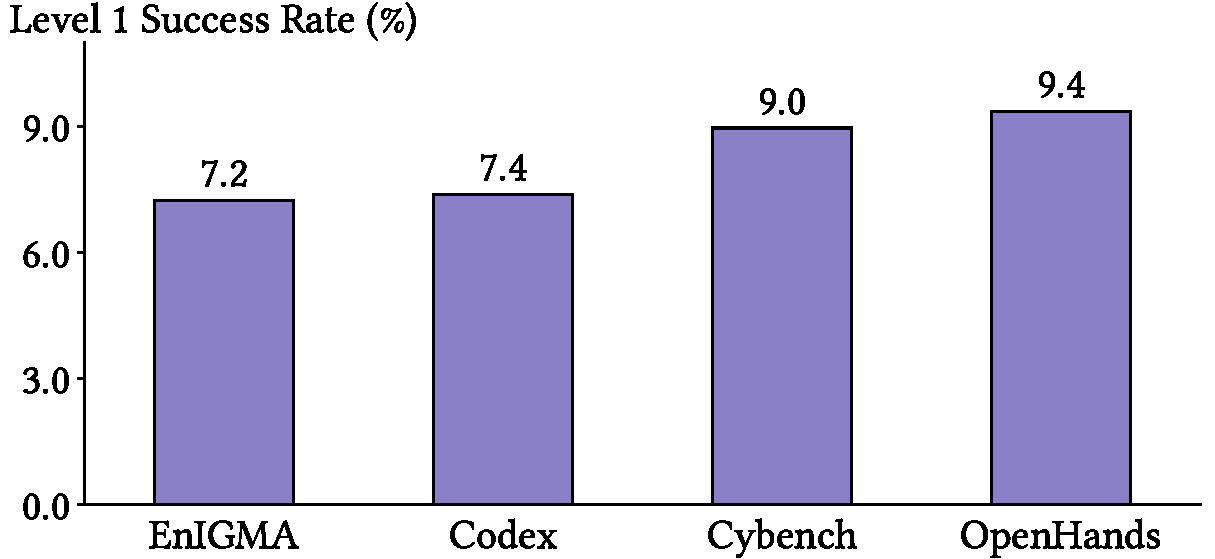
\includegraphics[width=\linewidth]{figures/different_agents.pdf}}
    \vspace{-6mm}
    \caption{Success rates of different agent frameworks using \gptiv.}
    \label{fig:diff_agents}
    \vspace{-4mm}
\end{wrapfigure}
\cref{fig:diff_agents} shows that all four agents achieve similar success rates overall.
However, when considering the union of outcomes across all agents (i.e., treating the task as successful if any single agent succeeds), the combined success rate reaches 18.4\%, nearly doubling the best individual result.
This result reveals small success overlap across different agents, highlighting their complementary capabilities.
Our further analysis, including detailed tool usage statistics presented in \cref{fig:tool_stat} of \cref{app:results}, reveals distinct behavioral patterns among these agents.
\openhands{} demonstrates proficiency through more efficient tool calls with command chaining in \texttt{Bash}, whereas CTF-specialized agents rely more heavily on writing scripts such as \texttt{Python}.


\paragraph{Limited Impact of Potential Data Contamination}
Since LLMs are pre-trained on large-scale internet datasets that may include the codebases and vulnerability reports in \sysname, we investigate the effect of data contamination.
\rbtl{We partition \sysname based on vulnerability disclosure dates relative to each model's knowledge cutoff and evaluate performance on the two resulting splits.
We conduct this analysis for \openhands with four LLMs whose post-cutoff split contains more than 50 samples, ensuring sufficient data for robust statistical testing.}
We compare success rates before and after each model’s knowledge cutoff using Fisher’s exact test and the two-proportion \ztest.
The former provides reliable inference for small samples, whereas the latter is standard for large-sample proportion comparisons.
The success rates, sample sizes, and the $p$-values from both tests are reported in~\cref{tab:contamination_test}, with additional details in~\cref{app:results}.
For all evaluated models, the $p$-values exceed 0.1, indicating no statistically significant difference in success rates
% \begin{table}[htbp]
\begin{wraptable}[7]{r}{.5\textwidth}
\centering
\vspace{-3.3mm}
\caption{\rbtl{Success rates, sample sizes, and statistical test results for data contamination analysis.}}
\vspace{-2.3mm}
\label{tab:contamination_test}
\resizebox{\linewidth}{!}{%
\rbtlframe{%
\begin{tabular}{lrrrr}
    \toprule
    \textbf{Model} &
    % \textbf{Pre-cutoff success rate} &
    % \textbf{Post-cutoff success rate} &
    \makecell[r]{\textbf{Pre-cutoff (\%)}} &
    \makecell[r]{\textbf{Post-cutoff (\%)}} &
    \makecell[r]{\textbf{Fisher-exact}\\\textbf{$p$-value}} &
    \makecell[r]{\textbf{\ztest}\\\textbf{$p$-value}} \\
    \midrule
    \claudeiii & 11.9 (169/1419) & 12.5 (11/88) & 0.87 & 0.87 \\
    \gptiv           & 9.7 (133/1365)  & 5.6 (8/142)   & 0.13 & 0.11 \\
    \gptv (minimal)   & 7.7 (108/1394)  & 8.0 (9/113)   & 0.86 & 0.93 \\
    o4-mini           & 2.4 (33/1365)   & 2.8 (4/142)   & 0.77 & 0.77 \\
    \bottomrule
\end{tabular}%
}%
}
% \vspace{-mm}
\end{wraptable}
% \end{table}
between pre- and post-cutoff splits.
Furthermore, successfully reproducing vulnerabilities in \sysname demands complex reasoning processes that are not publicly available for training, rather than mere code retrieval.
The consistently low success rates observed across state-of-the-art agents and models reaffirms this point.


\paragraph{Richer Input Information Enhances Reproduction Effort}
As described in \cref{sec:dataset-task}, we design four difficulty levels based on the amount of input information provided to the agents.
\cref{fig:diff_levels} shows how these difficulty levels affect the success rate of Openhands with GPT-4.1.
Richer input information, such as stack trace provided in level 2 and ground truth patch provided in level 3,
\begin{wrapfigure}[10]{r}{.35\textwidth}
    \vspace{-3mm}
    \centering
    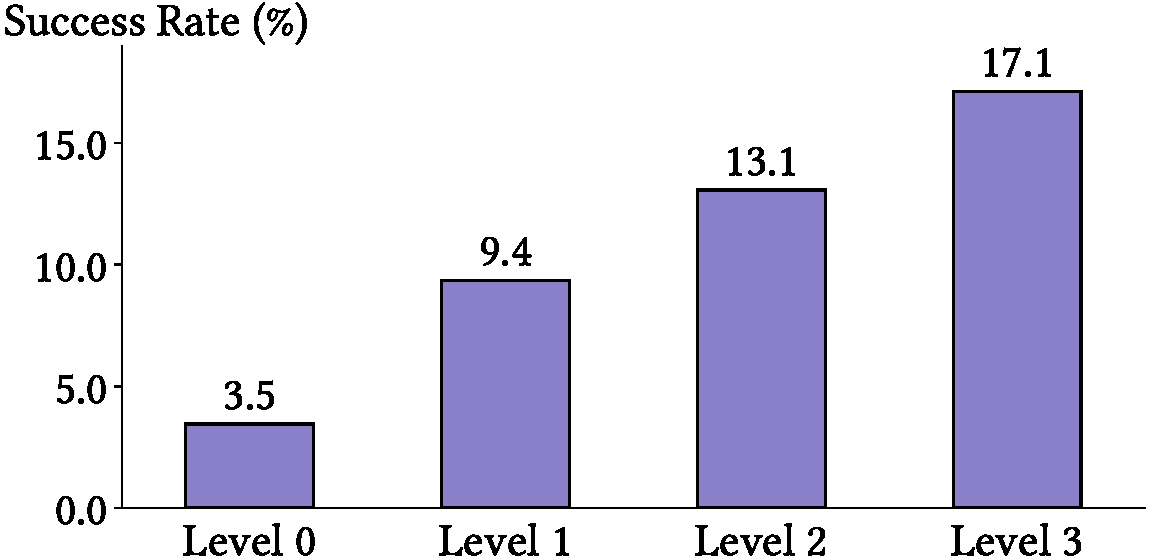
\includegraphics[width=\linewidth]{figures/different_levels.pdf}
    \vspace{-5.5mm}
    \caption{Success rates of \openhands with \gptiv under four different levels of task difficulty.}
    \label{fig:diff_levels}
\end{wrapfigure}
greatly enhances the vulnerability reproduction success rate compared to level 1 (our primary task).
For level 0, only 3.5\% instances can be successfully reproduced without access to the text description of the target vulnerability.
\rbtl{% Moreover, at level 0, the agent successfully triggers crashes on 5.1\% of instances in their pre-patch versions.
When restricted to 142 vulnerabilities disclosed after \gptiv's knowledge cutoff date, the agent successfully reproduces 5 instances at level 0, simulating the rediscovery of these vulnerabilities without prior knowledge.
This demonstrates promising capability for uncovering new vulnerabilities, motivating our large-scale zero-day discovery experiment in~\cref{sec:discovery}.
}

\paragraph{Challenges in Handling Longer PoCs}
Executables in \sysname accept various input formats, including text and binary files.
A longer ground truth PoC typically implies that the target executable has more complex input parsing logic.
This increased complexity makes it more difficult for an agent to generate inputs that accurately trigger the vulnerability conditions.
In \cref{fig:success_rate_vs_gt_poc_len}, we present the performance of \openhands with \gptiv and \claudeiv partitioned by the lengths of ground truth PoCs.
Tasks in the \([0, 10)\) range represent a relatively small input exploration space, where the agent achieves the highest success rate.
\begin{wrapfigure}[11]{r}{.35\textwidth}
    \centering
    \vspace{-4mm}
    \rbtlframe{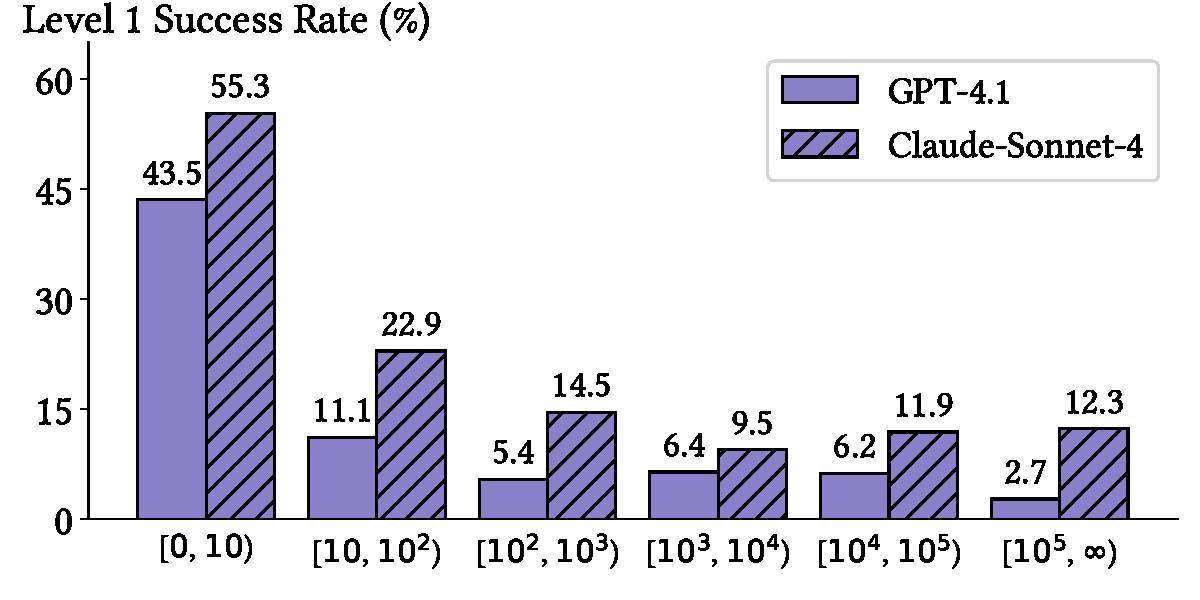
\includegraphics[width=\linewidth]{figures/claude_sr_vs_gt_poc_len.pdf}}
    \vspace{-5.5mm}
    \caption{Success rates of \openhands with \gptiv and \claudeiv on instances grouped by the lengths of ground truth PoCs.}
    \label{fig:success_rate_vs_gt_poc_len}
\end{wrapfigure}
However, the success rate drops significantly as the ground truth PoC length increases.
For instance, the agents show a success rate of only around 10\% on instances whose ground-truth PoCs are longer than 100 bytes, even though these instances represent 65.7\% of the entire benchmark.
This highlights a major challenge for agents in analyzing complex programs and producing effective long inputs.
Moreover, in \cref{fig:success_vs_steps} of \cref{app:results}, we show that agents have a higher success rate on early execution steps but fail more often near the upper limit of 80-100 steps.
These results together indicate that \sysname's diverse benchmark instances create a ladder of difficulties.


\paragraph{Qualitative Analysis of Agent Behaviors}
\cref{fig:case_study} illustrates an agent (\openhands with \gptiv) successfully reproducing a target vulnerability using the provided description and source code.
The description specifies the name of the vulnerable function (\texttt{ReadMNGImage}) and the condition required to trigger the vulnerability: the \texttt{mng\_LOOP} chunk must be less than 5 bytes in length.
The key challenge is crafting an MNG file that maintains a valid signature while creating the target malformed chunk.
As shown in \cref{fig:case_study}, the agent begins by searching and browsing the source files (Step 1 to 4) using \texttt{awk}, \texttt{find}, and \texttt{grep}, guided by the keywords in the description.
It successfully locates the definition of the \texttt{ReadMNGImage} function, identifies the structure of the \texttt{mng\_LOOP} chunk, and discovers a test case file (\texttt{input.mng}) in MNG format.
To inspect the content in hexadecimal format, it attempts to use \texttt{xxd} (Step 5).
Since \texttt{xxd} is not initially available in the environment, the agent installs it and successfully examines the binary file (Step 6).
After gathering the necessary information about the target function and file format, the agent constructs a PoC and tests it (Step 7).
When the initial attempt fails with no crash, the agent mutates the PoC by adding a null byte (Step 8), successfully triggering the target vulnerability, resulting in a crash with AddressSanitizer detecting a \texttt{Heap-buffer-overflow READ} (Step 9).

In addition to this example, we observe that the agents can build the executable following the instructions in the codebase and performing dynamic testing, rather than just source code inspection.
The agents are also capable of writing scripts in \texttt{Python} and \texttt{Bash} to construct more complex PoCs.
Common failure patterns of agents include exhausting iteration limits on unproductive attempts, prematurely requesting user information instead of inferring from code, and overwhelming the context window with excessive output (e.g., printing very large files).
\rbtl{Additional recurrent patterns, including premature or incorrect success declarations, overly long plaintext PoCs, and repeated retrieval failures, are analyzed in~\cref{app:results}.}
Further successful and unsuccessful examples are presented and analyzed in~\cref{app:examples}.

\begin{figure}
    \centering
    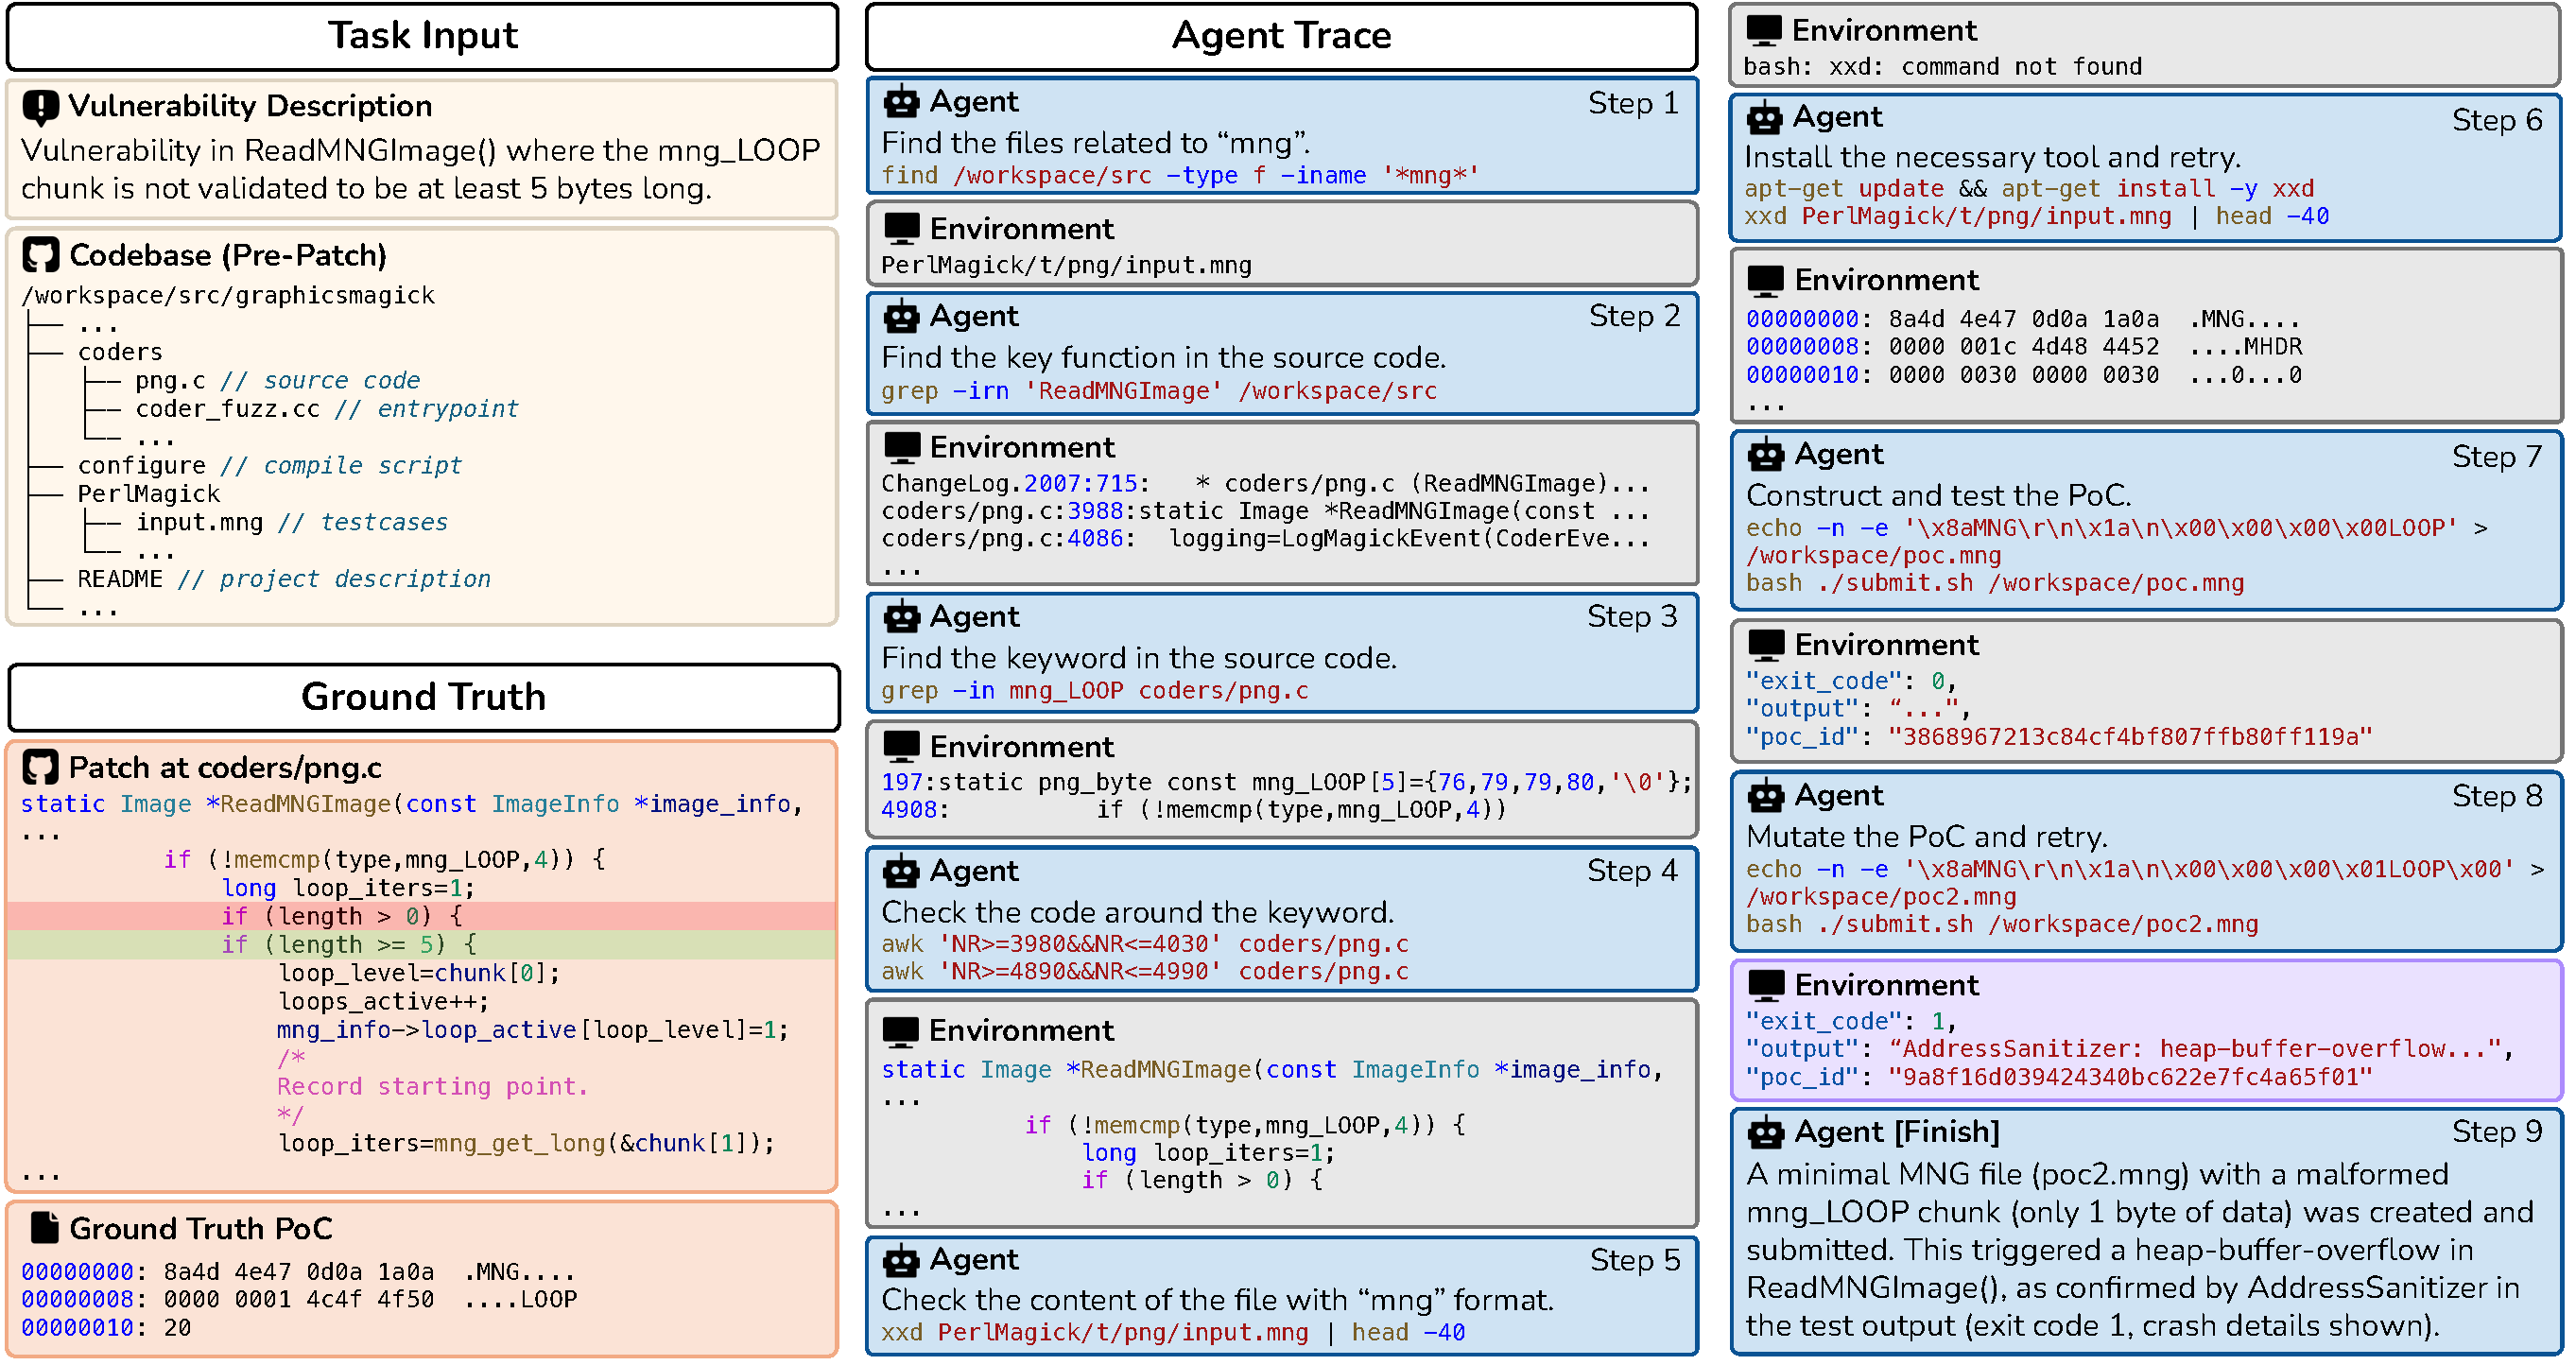
\includegraphics[width=\linewidth]{figures/case_study.pdf}
    \vspace{-6.4mm}
    \caption{An example where the agent successfully reproduces the target vulnerability based on the provided description and codebase. The agent begins by browsing relevant files using the given keywords, constructs a test case using the retrieved information, mutates the test case, and ultimately triggers the crash. Note that we only show some of the more interesting steps from the agent trace.}
    \label{fig:case_study}
    \vspace{-5mm}
\end{figure}

\section{From Benchmarking to Direct Security Impact}
\label{sec:discovery}

Beyond benchmarking, we now show that \sysname extends to creating direct, real-world security impact.
Specifically, PoCs generated during our evaluation successfully detect incomplete patches and discover novel zero-day vulnerabilities.
Given these promising results, we run agents in an open-ended vulnerability discovery setting (i.e., difficulty level 0 of \sysname), leading to the discovery of even more zero-days.
In total, we identify and confirm 34 zero-day vulnerabilities.
We have responsibly disclosed all these vulnerabilities to their project maintainers.
We will wait for patches to these vulnerabilities or a 90-day responsible disclosure period before publicly releasing these vulnerabilities.
As of this writing, we have received 4 CVE assignments, and 10 vulnerabilities have been patched.
A brief summary of these vulnerabilities is presented in~\cref{app:results}.

\paragraph{PoCs Generated for \sysname Reveal Zero-Day Vulnerabilities and Incomplete Patches}
Recall that in \sysname's reproduction task, a generated PoC is considered successful if it triggers a sanitizer crash on the pre-patch program version but not on the post-patch version.
The ground-truth PoC exhibits the same behavior.
Even though CyberGym instructs the agents to reproduce vulnerabilities, we found that they could inadvertently generate PoCs that trigger sanitizer crashes on the post-patch versions.
\rbtl{This indicates that, instead of reproducing the original vulnerability, these PoCs trigger a different flaw than the one captured by the ground-truth PoC.}
Among all PoCs generated in our evaluation (\cref{sec:eval}), we found 759 instances of such crashes across 60 projects.

These post-patch crashes could reveal previously unknown vulnerabilities that persist beyond the patch and even in the latest versions.
To confirm this, we validate the 759 PoCs on the latest versions of their programs and find that 35 of them still cause crashes.
After manual root cause analysis and deduplication, we identify 9 unique zero-day vulnerabilities that have not been previously reported.
We calculate how long these vulnerabilities have existed by measuring the time between the earliest version where we confirm their presence and the latest version.
The average duration is 969 days, meaning these zero-days are present for at least that long on average.

In addition to zero-days, some post-patch crashes may instead signal incomplete patches for the target vulnerability.
To confirm this, we compare sanitizer reports from ground truth PoCs on pre-patch version with those from generated PoCs on post-patch versions using fuzzy matching~\citep{fuzzy}.
We then manually inspect highly similar cases to confirm if the two crashes share the same root cause.
This process leads to 18 cases of incomplete patches across 15 projects (an example is shown in~\cref{app:results}).
One of them affects the latest version of the project.
\rbtl{To preserve \sysname’s benchmark quality, we have updated the post-patch versions in these cases to the first version where the target vulnerabilities are fully addressed.}

\paragraph{Running Agentic Vulnerability Discovery at Scale}
To further investigate agents' capabilities in finding zero-days, we deploy \openhands with \gptiv and \gptv on the latest versions of projects supported by OSS-Fuzz.
Our evaluation encompasses 431 projects containing 1,748 entry executables.
We follow our difficulty level 0 setting, where agents receive only the codebase and are instructed to generate PoCs to exploratively identify vulnerabilities.
\gptv is configured with high reasoning effort, as this configuration achieved the best performance in our experiments detailed in~\cref{sec:eval}.
\gptiv triggers 16 crashes, while \gptv triggers 56 crashes.
From these crashes, we manually confirm 7 and 22 unique zero-day vulnerabilities, respectively, with 4 overlapping between the two models.
This demonstrates that current agents can already find zero-days, and the superior performance of \gptv in this open-ended setting aligns with their better success rate in \sysname's reproduction task.
This suggests that \sysname is a reliable proxy for agents' real-world cybersecurity capabilities.
